\section{Software Realization}
\label{sec:software-realization}
To fully understand and verify the ADRIAN protocol \cite{mann2023ADRIAN}, we have to implement a prototype of the protocol. This section describes the design and implementation of the software system that implements the ADRIAN protocol, as well as the experimental setup used to evaluate the protocol. The implementation is done in Java, and the source code can be found on GitHub\footnote{\url{https://github.com/jornverhoeven/thesis-project}}. 


\subsection{Overview}
\label{ssec:overview}
% \comment{Zoltan}{It would be a good to add an overview diagram that shows the structure of the while program on a higher level of abstraction than individual classes.}
To start things off we will give a brief overview of the components of the ADRIAN prototype. The component overview can be seen in Figure \ref{fig:adrian-component-overview}, and will be used as a reference throughout this section.

\begin{figure}[H]
    \centering
    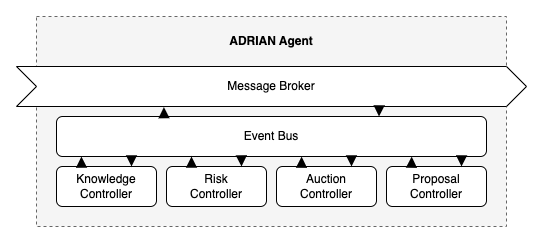
\includegraphics[width=0.8\textwidth]{_content/adrian-component-overview.png}
    \caption{Simplified overview of the components of the ADRIAN prototype. The \code{Message Broker} is responsible for interfacing with the external world, while the \code{Event Bus} is used for internal communication. The \code{Controllers} are responsible for handling the different aspects of the agent, such as knowledge sharing and auctions. They are each responsible for a specific set of events and are connected to the \code{Event Bus}.}
    \label{fig:adrian-component-overview}
\end{figure}

For the architecture design of the prototype, the goal was to create something that is easy to understand, maintain, and instrument. To achieve this, the decision was made to implement an Event-Driven architecture. This architecture is based on the Observer pattern \cite{gamma1995design}, commonly used in software development. By sending messages through an event bus (See \code{Event Bus} in Figure \ref{fig:adrian-component-overview}), it is possible to decouple the different components of the system. Next to being able to decouple the components, it also allows us to easily instrument the system. By listening to the events on the event bus during our experiments, it is possible to count the number of events and the time between events. This allows us to easily collect metrics of the system. More on these metrics in Section \ref{ssec:metrics}.

Each controller in our design is responsible for a specific set of events and is connected to the event bus. This allows us to easily add new controllers, or replace existing ones during our experiments. The controllers are responsible for handling the different aspects of the agent. 

\begin{enumerate}
    \item The \code{KnowledgeController} is responsible for receiving and sharing knowledge. 
    \item The \code{RiskController} is responsible for detecting risks.
    \item The \code{AuctionController} is responsible for handling auctions. 
    \item The \code{ProposalController} is responsible for finding and applying proposals.
\end{enumerate}

The decision was made to detach the external communication from the internal communication. External being the communication to other agents, and internal the communication within the agent itself. This allows for easier replacement of the external communication with a different implementation. More on this in Section \ref{sssec:message-broker}.
The \code{Message Broker} is the layer for interfacing with the external world, and is responsible for sending and receiving messages from other agents and dispatching them to the event bus.

\subsection{Class Diagrams}
\label{ssec:class-diagrams}
\addtocontents{toc}{\protect\setcounter{tocdepth}{2}}

In this section, we present an overview and analysis of a UML Class Diagram for our proposed implementation of the ADRIAN protocol which can be seen in Figures \ref{fig:uml-agent} through \ref{fig:uml-services}. At a glance, the architecture features multiple controllers, connected through an internal event bus, and a message broker which enables external communication. Additionally, some classes have been extended to support the experimental setup, which is further explained in Section \ref{sec:experiments}.

\begin{figure}[H]
    \centering
    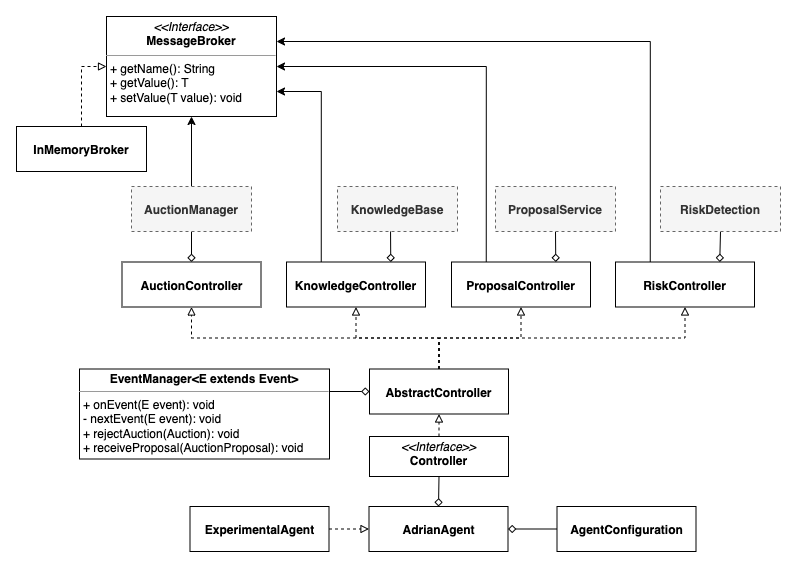
\includegraphics[width=1.0\textwidth]{_content/uml-agent}
    \caption{UML Diagram of the code structure of an Agent.}
    \label{fig:uml-agent}
\end{figure}

\subsubsection{Increased Cohesion and Reduced Coupling through Controller Interfaces}
\label{sssec:reduced-cohesion-coupling}
The systems architecture uses multiple controllers to handle various aspects of the agent, aiming to increase cohesion and reduce coupling between components. Each controller is responsible for a specific set of tasks and the corresponding events, leading to a more modular and flexible design. This separation of functionality allows for easier maintenance, as well as the ability to replace controllers with new implementations, minimizing the impact on other parts of the system. One place where this modularity is especially useful is in the experimental setup, where we enable or disable certain features of the agent by replacing the controllers with different implementations. For example, we can disable the \code{AuctionController} by replacing it with a \code{ProposalImplementation\-Controller}, this can then bypass the auction logic and choses the best proposal by itself. This allows us to easily test the system without auctions, and compare the results with the system with auctions enabled.

\subsubsection{Event Bus for internal communication}
\label{sssec:event-bus}
To enable communication between controllers, an internal event bus is created. The event bus is in essence nothing more than the implementation of the Observer pattern (also known as \texttt{EventEmitter} or \texttt{Pup/Sub})\cite{gamma1995design}. This decouples the controllers from one another, as they are not directly aware of each other. Controllers can publish and subscribe to events on the event bus, and the event bus will then notify all subscribers when an event is published. These events can also be listened to during the experiments, allowing us to capture metrics such as the amount of risks detected, auctions started and more. More on these metrics in Section \ref{ssec:metrics}.

\subsubsection{Controllers as an interfacing layer}
\label{sssec:controllers-interfacing-layer}
Controllers serve as an interfacing layer, between the event bus and the services responsible for the computations. They essentially serve as a translator between events and the logic implemented by the services. This abstraction shields the services from the complexities of event handling, promoting modularity and reusability. It allows the services to be reused in other contexts and makes the code easier to test as the services it uses are not dependent on any external form of communication.

\subsubsection{Message Broker for external communication}
\label{sssec:message-broker}
The system uses a \code{MessageBroker} which facilitates communication between agents. It allows for both incoming and outgoing messages to be handled by the agent while abstracting away the underlying (networking) protocol. Incoming messages are processed and dispatched onto the internal event bus, triggering the relevant controllers to handle the message. On the other hand, outgoing messages are sent to the \code{MessageBroker}, which then sends the message to the appropriate agent.

For our simulation we chose to implement the \code{MessageBroker} as a simple in-memory message broker. No actual HTTP request or other protocol is used, as all agents run on the same machine. This allows us to easily simulate the network communication, without having to worry about the complexities of the network. In a real-world scenario, the \code{MessageBroker} would be a network service, which is used to send messages between agents over the network using HTTP requests or some other protocol such as MQTT. From the agent's perspective, the \code{MessageBroker}'s interface would be the same, regardless of the concrete implementation.


\subsubsection{Similarities in graph data structures}
\label{sssec:graph-data-structures}
In the real world, the infrastructure is a graph structure. When instantiated, an agent get access to information about its hosting node, and the unique identifiers (ID's) from its neighboring nodes. From its hosting node, the agent can access to all properties and use those properties to create the initial knowledge base. The \code{Infrastructure}-graph consists of two types of nodes; \code{InfrastructureNode} and \code{SoftwareComponent}. These nodes can be mapped to actual hardware (e.g. servers and IoT devices) and software (e.g. databases and services) in real-world applications. For this software implementation it was decided to omit the concrete implementation of these classes such as \code{Database} or \code{IoTDevice}, as the \code{InfrastructureNode} and \code{SoftwareComponent} are sufficient for the purpose of this thesis. Moreover, adding the concrete implementations would most likely only confuse the reader, as the concrete implementations are not relevant to the ADRIAN protocol.

\begin{figure}[H]
    \hspace*{-1cm}     
    \centering
    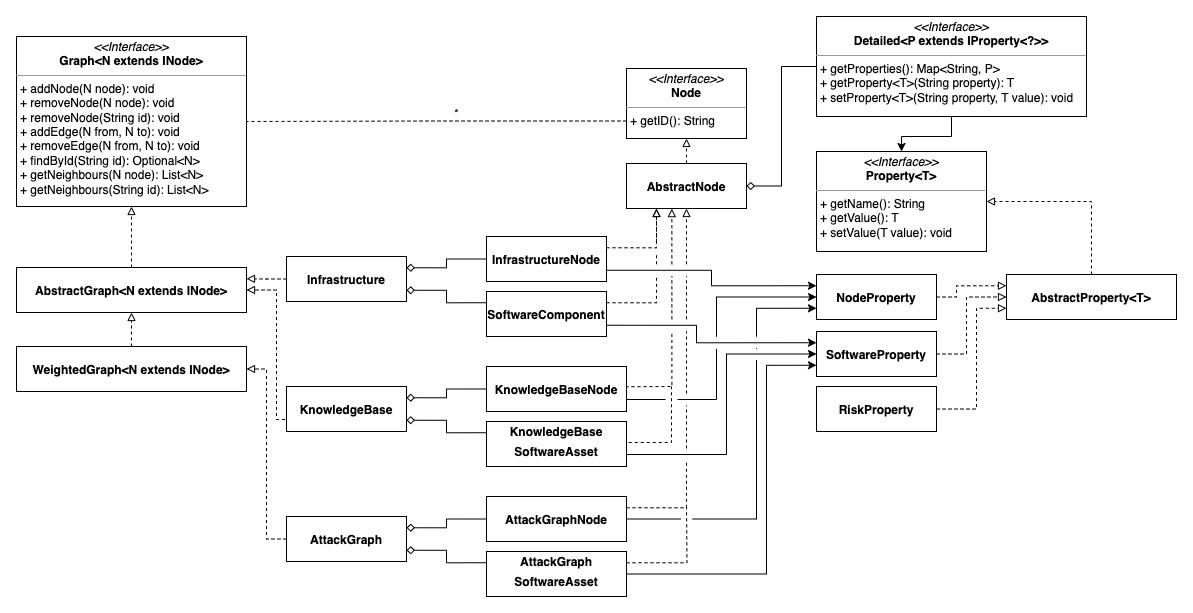
\includegraphics[width=1.2\textwidth]{_content/uml-graphs}
    \caption{UML Diagram explaining the structure of the graphs, where the \code{Infrastructure} graph is the graph used to represent the actual infrastructure of the experiment. The \code{KnowledgeBase} graph is the graph used to represent the knowledge of the agent. The \code{AttackGraph} is the graph used to represent risks found by the agent in its knowledge base.}
    \label{fig:uml-graphs}
\end{figure}

Throughout the runtime of the application agents learn knowledge from other agents. The concept by Mann and Smolka\cite{mann2023ADRIAN} mentions that every piece of information in the knowledge base has a timestamp from when it originated. However, when the initial streams of communication between agents started some race conditions appeared, causing incorrect/mismatched data to flow into the system. To overcome issues with overwriting an agents information a tiered knowledge system has been implemented using Java's enumerate classes. A \code{KnowledgeOrigins}-enumerate has been created which we have split into three options. The knowledge each agent knows about the host-node (properties) is called \emph{Direct-knowledge}, and the information about connected nodes from the start is called \emph{Inferred-knowledge} (because the agent knows something should be there, but not exactly what). During the execution of the experiments an agent it will learn more about agents and nodes around it, and this information is called \emph{Indirect-knowledge}. When an agent learns something from another agent, it will store the information in its knowledge base. This allows us to easily keep track of where the information came from, and if it is still relevant. For example, an agent will never overwrite its \emph{Direct-knowledge} with \emph{Indirect-knowledge}, as \emph{Direct} is more reliable. However, it will overwrite \emph{Inferred-knowledge} with \emph{Indirect-knowledge} as \emph{Inferred} is only the indication that there should be some value but is unknown what that is exactly.

\subsubsection{Services}
\label{sssec:services}
Each controller is only responsible for converting events into service calls. But to implement the actual logic, the controllers use services. These services are responsible for the actual computations, such as calculating the \code{AttackGraphs} or finding \code{Proposal}s. Figure \ref{fig:uml-services} shows how the services are tied together.

\begin{figure}[H]
    \centering
    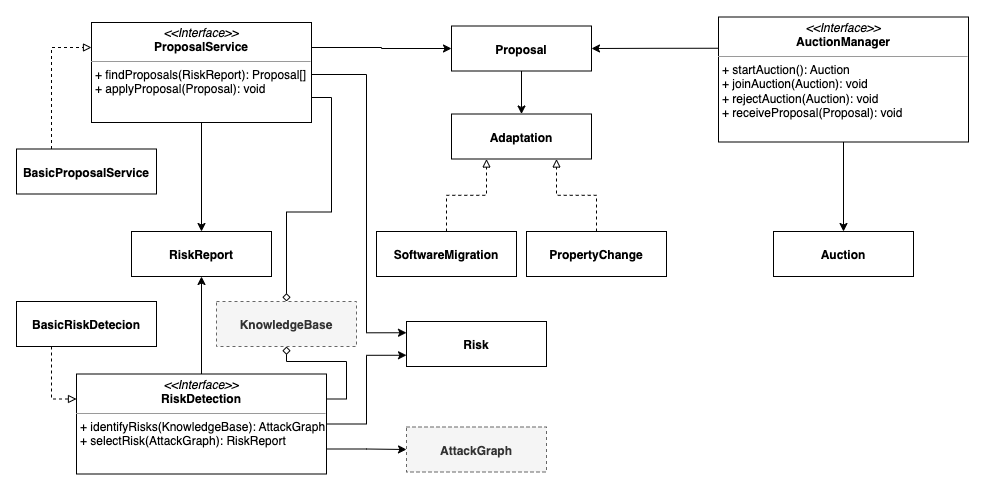
\includegraphics[width=1.0\textwidth]{_content/uml-services}
    \caption{UML Diagram depicting how the agent's services are tied together. The \code{ProposalService}, \code{RiskDetection}, and the \code{AuctionManager} are the three main services that are used by the agent. The \code{BasicProposalService} and \code{BasicRiskDetection} are the default implementations of the services.}
    \label{fig:uml-services}
\end{figure}

\begin{description}
    \item[RiskDetection] This service is responsible for detecting risks in the infrastructure. It does this by generating the attack graph from the agents knowledge base. With the attack graph, it can then identify \textit{Critical Paths} by finding paths from nodes that are exposed to the outside and ending at a \textit{critical software component}. These \textit{Critical Paths} are then used to calculate the risk damage value. For each critical path we calculate the risk damage value by taking the potential damage value of the critical software component (at the end of the path) and multiplying it by the probability of the path. The probability is calculated as described in Section \ref{ssec:risk}. The result of this operation is called the \emph{risk report}. Figure \ref{fig:attack-graph-to-risk-report} shows an example of the difference between an attack graph and a risk report. In this figure we see a representation of the attack graph on the left, showing the multiple risks (edges) between nodes with their individual weights. Risk-edges are directional and can go in multiple directions, as shown in the example. On the right we see the risk report, which is a simplified version of the attack graph. It only shows the edges that are in the same direction as the critical path. This is done to simplify the risk report, and to make it easier to calculate the risk damage value. The risk report is directional, and can have incoming edges to indicate that a node could be the starting point of an attack. The risk report is then used to start an auction, which is explained in Section \ref{ssec:auctions}.
    
    \begin{figure}[H]
        \label{fig:attack-graph-to-risk-report}
        \centering
        \begin{subfigure}[b]{0.4\textwidth}
            \centering
            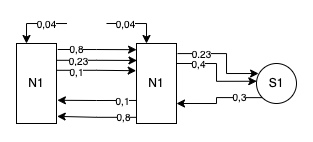
\includegraphics[width=\textwidth]{_content/attack-graph.png}
            \caption{Attack graph between nodes and software components}
            \label{fig:attack-graph}
        \end{subfigure}
        \hspace{0.5cm}
        \centering
        \begin{subfigure}[b]{0.4\textwidth}
            \centering
            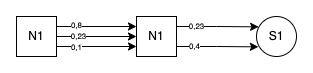
\includegraphics[width=\textwidth]{_content/riskreport-future-research-a.png}
            \caption{Risk report for a critical path}
            \label{fig:risk-report}
        \end{subfigure}
        \caption{On the left is the graph representation of an attack graph, where each edge is a risk that holds a probability of an attacker exploiting it. The graph is directional and can hold edges in multiple directions. On the right is the graph representation of a risk report. The risk report is also directional but only contains the edges that are in the same \textit{direction} as the critical path. Both graphs can have incoming edges to indicate that a node could be the starting point of an attack.}
    \end{figure}



    \item[ProposalService] This service is responsible for calculating proposals that the node is able to apply. It does this by taking the risk report from an auction and merging it in its own knowledge base to update it with the latest information about the risk. It will then apply different adaptations to a copy of the knowledge base. An adaptation could be, for example, to update the properties of a node or software (Refer to Section \ref{ssec:risk-rules-adaptaions} for more information). From this adaptation to the copied knowledge base, the service can recalculate the risk damage value for the critical path. From the list of all applicable adaptations, the adaptation that mitigates the risk and reduces the damage the most is selected. Additionally, the agent checks if the adaptation does not introduce any new risks. More on that in Section \ref{ssec:risk-deltas}. The selected adaptation is then used as a bid in the auction, for the auctioneer to consider. 
    
    \item[AuctionManager] This service is responsible for starting and managing the auction state of an agent. Once the \code{RiskDetection} selects a risk to mitigate, the \code{AuctionManager} will start a new auction. It will send invitations to other agents and wait for their replies (accept or reject). It will also keep track of the current state of the auction and wait for proposals to be submitted. When a proposal is submitted, it will check if all participating nodes replied. If this is the case, it will calculate the risk damage value for each proposal, and select the proposal with the lowest risk damage value. This proposal is then broadcasted to all participating nodes, and the auction is finished. The manager will then wait for the next auction to start. There might also be cases where participating nodes fail to send proposals. For these cases, the \code{AuctionManager} has a timeout that starts when an auction starts. If the timeout is reached, the manager will finish the auction at that point, and select the proposal with the lowest risk damage value. If no applicable proposals are received, the auction is canceled and nothing is done. 
    
    For agents that are participating, and not the auctioneer, the \code{AuctionManager} will ensure that an agent can only join a single auction at a time. This is done to prevent an agent from joining multiple auctions at the same time, and potentially having to apply multiple adaptations at the same time. This could lead to a situation where an agent has to apply adaptations that are incompatible with each other. For example, an agent could receive two proposals to migrate software from one node to another. However, the software that is being migrated is the same in both proposals. This would lead to a situation where the agent would have to migrate the software to two different nodes at the same time, which is not possible. To prevent this, the \code{AuctionManager} will only allow an agent to join a single auction at a time. If an agent is already participating in an auction, it will reject any new invitations to join an auction. 

\end{description}

% \subsection{Sequence Diagrams}
% \label{ssec:sequence-diagrams}
% \add{Update text or remove section}
% \begin{figure}[H]
%     \centering
%     \includegraphics[width=0.8\textwidth]{_content/knowledge-sharing}
%     \caption{Knowledge Exchange Sequence Diagram}
%     \label{fig:knowledge-sharing}
% \end{figure}

% \begin{figure}[H]
%     \centering
%     \includegraphics[width=0.8\textwidth]{_content/auction}
%     \caption{Auction Sequence Diagram}
%     \label{fig:auction}
% \end{figure}

% \addtocontents{toc}{\protect\setcounter{tocdepth}{3}}

\subsection{Risk Rules \& Adaptations}
\label{ssec:risk-rules-adaptaions}
In this section risk rules and adaptations that are used in the ADRIAN protocol \cite{mann2023ADRIAN} will be explained. The risk rules are used to identify risks in the infrastructure. These rules are based on the different properties of the infrastructure and software components, and they can represent a risk between two nodes, regardless of whether it is an infrastructure node or software component.

To implement the risk rules it was decided to distinguish between three types of risks; \emph{Forward risks}, \emph{Backwards risks}, and \emph{Inward risks}. Figure \ref{fig:risk-rules} gives a visual representation of the differences between these three types of risks. 
\emph{Forward risks} are risks that are triggered by a property (or combination of properties) on the parent node. They create a directed edge from the parent node to the child node. 
\emph{Backwards risks} are risks that are triggered by properties on the child node. They create a directed edge from the child node to the parent node. 
\emph{Inward risks} are risks that are triggered by properties on a node. They create a directed incoming edge to the child node. To implement incoming edges, we use a \emph{void node}, as is also shown in Figure \ref{fig:risk-rule-inward}. The void node is a node that is not part of the infrastructure, and is only used to represent incoming edges.
\emph{Inward risks} are nearly identical to \emph{Backwards risks}, the only theoretical distinction is that inward risks always come from a void-node, whereas backwards risks only come from entities on the graph. 
The choice to split the risks rules into these three types is based on the way each rule checks the knowledge base, and is purely a technical distinction. They each have small differences in the way they loop over the knowledge base, and how they check for specific properties.

\begin{figure}[H]
    \begin{subfigure}[b]{0.3\textwidth}
        \centering
        \includegraphics[width=\textwidth]{_content/risk-rules-forward.png}
        \caption{Forward risk rule.}
        \label{fig:risk-rule-forward}
    \end{subfigure}
    \begin{subfigure}[b]{0.3\textwidth}
        \centering
        \includegraphics[width=\textwidth]{_content/risk-rules-backward.png}
        \caption{Backwards risk rule.}
        \label{fig:risk-rule-backward}
    \end{subfigure}
    \begin{subfigure}[b]{0.3\textwidth}
        \centering
        \includegraphics[width=\textwidth]{_content/risk-rules-inward.png}
        \caption{Inwards risk rule.}
        \label{fig:risk-rule-inward}
    \end{subfigure}
    \caption{A representation of the three different risk rules. The asterisk (*) represents a property that would trigger the risk rule. The arrows represent the direction of the risk. Any square could be either a node or a software component. In the case of Inward rules, the parent will always be the void node.}
    \label{fig:risk-rules}
\end{figure}

These three types of risks are then used to implement the different risk rules. The risk rules are made up partially from existing CVE's, but also from theoretical risks that could occur in a real-world scenario, such as not having a firewall. These theoretical risks are used to further test the system, and show that the system is not just limited to CVE's that are known at the time of implementation. The risk rules used throughout this thesis are shown in Table \ref{table:risk-rules}. A production ready version of the system would likely include a larger set of risk rules, and would be updated regularly to include new CVE's. However, for the purpose of this thesis, we have chosen to limit the amount of risk rules to a small set of rules.

In Table \ref{table:risk-rules} the adaptations that the agent could used to mitigate the risks are also shown. These adaptations are used to reduce the risks in the infrastructure. The ADRIAN concept \cite{mann2023ADRIAN} mentions two types of adaptations, \emph{Property Change} and \emph{Migration}. Both of these are implemented in the proof of concept. The adaptations in Table \ref{table:risk-rules} are split into \emph{Enable Property} and \emph{Version Change}, both of which are \emph{Property Change} adaptations. Enabling a property is used for boolean properties such as \emph{hasFirewall} and \emph{isSoftwareEncrypted}, which are the properties used by the risk rules. \emph{Version change} is used for version properties, and follow a Semantic Version scheme\footnote{\url{https://semver.org/}}. This distinction is made to show that the adaptations are not limited to a single type of property, and that the system is able to handle different types of properties.

The current software implementation has a one-to-one relation between an adaptation and the risk it mitigates. This means that an individual risk only has (at most) a single possible adaptation. Conceptually, this should not change or influence the experiment, as the additional adaptations would be added to the list waiting to be evaluated like the others. Something that is not trivial from Table \ref{table:risk-rules} and the description above is that a single adaptation could potentially solve multiple risks. For example, multiple risks could rely on the same SDK-version, which is resolved in both cases by the same new version. For the experiments in this thesis, this scenario does not occur, to keep the experiments simple. However, in a real-world scenario, this could be a more common occurrence.

% \comment{Zoltan}{This table gives the impression that there is a 1-1 correspondence between risk rules and adaptations. This is not the case, as the same adaptation can be used to mitigate multiple risks and vice versa.}
% \comment{Zoltan}{Give an example of a workedout risk rule, and its implications in the real world + the adaptation that is used to mitigate it.}
\begin{table}[H]
    \centering
    \begin{tabular}{l|l|l|l|l}
        \textbf{Name} & \textbf{Rule Type} & \textbf{$\mathbf{p}_{\mathbf{k}}$} & \textbf{Adaptation} & \textbf{\begin{tabular}[c]{@{}l@{}}Mitigation \\ Probability\end{tabular}} \\ \hline
        \textbf{Uncertainty} & Inward & $0.08$ & N.A. & \\
        
        \textbf{Firewall} & Backward & $0.8$ & Enable Property & $0.2$ \\
        \textbf{Physically Secured} & Backward & $0.8$ & Enable Property & $0.2$ \\
        \textbf{Software Encrypted} & Backward & $0.8$ & Enable Property & $0.2$ \\
        
        \textbf{CVE-2020-3676} & Forward & $0.18$ & Version Change & $0.0$ \\
        \textbf{CVE-2021-22547} & Forward & $0.18$ & Version Change & $0.0$ \\
        \textbf{CVE-2021-40830} & Inward & $0.28$ & Version Change & $0.0$ \\
        \textbf{CVE-2022-25666} & Forward & $0.08$ & Version Change & $0.0$ \\
        \textbf{CVE-2022-35927\tablefootnote{\label{cve-2022-35927} This CVE introduces both a backward and inward risk.}} & Backward & $0.39$ & Version Change & $0.0$ \\
        \textbf{CVE-2022-35927\footnoteref{cve-2022-35927}} & Inward & $0.39$ & Version Change & $0.0$ \\
        
        \textbf{Firmware Risk\tablefootnote{\label{cve-test-risk} These risks are used for testing and are made up, and thus they have no real-world parallel }} & Forward & $0.1$ & N.A. & \\
        \textbf{OS Risk\footnoteref{cve-test-risk}} & Forward & $0.4$ & Version Change & $0.0$ \\
        \textbf{SDK Risk\footnoteref{cve-test-risk}} & Forward & $0.99$ & Version Change & $0.0$ \\
    \end{tabular}
    \caption{\label{table:risk-rules}Overview of the implemented risk rules. It shows the name or identifier for each rule, the type of rule, the risk probability, the adaptation that is applied to mitigate the risk, and the mitigation factor that is used to calculate the new risk probability.}
\end{table}

One example of one of the risks from Table \ref{table:risk-rules} would be the following: \href{https://nvd.nist.gov/vuln/detail/CVE-2022-35927}{CVE-2022-35927}.
This risk is a vulnerability in the Contiki-NG operating system, which is used in IoT devices. The vulnerability allows an attacker to perform a buffer overflow attack\footnote{More information about Buffer Overflows can be found here \url{https://en.wikipedia.org/wiki/Buffer_overflow}}. According to the CVE, the vulnerability is present in any version prior to version $4.7$. The suggested adaptation to mitigate this risk is to update the version of the operating system to version $4.7$ or higher. This is a \emph{Version Change} adaptation, and is used to mitigate the risk. The risk rule for this risk is a \emph{Forward} risk rule, as the risk is triggered by a property on the parent node (the operating system), and affects the child nodes connected to it. The risk probability is set to $0.39$, which is the probability of an attacker exploiting the vulnerability. This probability is based on the exploitability-score which is given for the CVE, in this case $3.9$. The mitigation factor is set to $0.0$, as the risk is completely mitigated by updating the operating system.  

% \comment{Jorn}{Explain the uncertainty risk}
% \tablefootnote{We always include a small risk to incorporate the uncertainty factor, and allow agents to detect additional risks which would otherwise be hidden. }
One of the risk rules that is implemented is the Uncertainty-risk. This risk is used to incorporate the uncertainty factor, and allow agents to detect additional risks which would otherwise be hidden. If this risk would be omitted, it would be possible for certain scenarios to occur where an agent would not be able to detect any risks. One example of this would be a scenario where there is no risk from a node ($A$) to a critical software component (hosted on $A$). However, there could be a risk from a node $B$ to $A$. This is illustrated in Figure \ref{fig:uncertainty-infrastructure}. If the Uncertainty-risk would be left out, $B$ would not be able to create a critical path through $A$ to the critical software component, as is depicted in Figure \ref{fig:uncertainty-attack}. This would mean that the agent would not be able to detect the risk, and would not be able to mitigate it. By including the Uncertainty-risk, the agent would be able to find the critical path, and thus be able to mitigate the risk.

\begin{figure}
    \begin{subfigure}[b]{0.47\textwidth}
        \centering
        \includegraphics[width=\textwidth]{_content/uncertainty-infrastructure.png}
        \caption{Simplified infrastructure depicting the connections between two nodes (A and B) and a software component (S).}
        \label{fig:uncertainty-infrastructure}
    \end{subfigure}
    \hfill
    \begin{subfigure}[b]{0.47\textwidth}
        \centering
        \includegraphics[width=\textwidth]{_content/uncertainty-attack.png}
        \caption{The attack graph between two nodes (A and B) and no risks towards the software component (S).}
        \label{fig:uncertainty-attack}
    \end{subfigure}
    \caption{A simplified representation of an infrastructure, to illustrate the effect of the uncertainty risk. (a) Shows the simplified infrastructure. (b) shows the attack graph between two nodes (A and B) and no risks towards the software component (S).}
    \label{fig:uncertainty}
\end{figure}

\subsection{Migrations} 
\label{ssec:migrations}
Whereas Table \ref{table:risk-rules} shows all implemented risk rules, and their potential adaptations, it does not show the migrations an agent can make. This is due to migrations not being tied to any specific risk rule, but rather to the infrastructure itself. This means that migrations are not triggered by an individual risk rule. Instead, migrations are attempted and evaluated by the \code{ProposalService} (see Section \ref{sssec:services}) based on the critical path, the critical software, and the agent itself. This does not mean that migrations are not related to risks at all. In fact, migrations are used to mitigate risks, and are evaluated based on the risk damage value. However, the decision to migrate software is not based on a single risk rule, but rather on the overall risk damage value of the critical path.

While developing and experimenting with the ADRIAN protocol, we noticed that the mitigation strategy to migrate software from one node to another is seldom applied. Only under special circumstances will the agents propose to migrate software from one node to another. To illustrate some of the reasons why this is the case, we will sketch several cases that were encountered during the experiments, and why the agents did not \emph{(and should not)} propose to migrate software.

\paragraph*{Migrating along the critical path}
In Figure \ref{fig:migrations-infrastructure} we see a simplified infrastructure. The critical path from node A to software S1 is shown in red. If we were to migrate software S1 to node A, the critical path would be shortened as shown in figure \ref{fig:migrations-shortened}. None of the properties change and all edge-probabilities stay the same. Only the critical path changes. This means that the damage value would in almost all cases increase, as any additional edges (unless the probability is exactly 1) decrease the probability of an attacker reaching the critical component, because each probability is always \(0 \leq p \leq 1\). 

The migration would be beneficial only if the new edge between node A and software component S1 has a significantly reduced probability. However, because the properties of A and S1 do not change, this is unlikely to happen.

\begin{figure}[H]
    \begin{subfigure}[b]{0.3\textwidth}
        \centering
        \includegraphics[width=\textwidth]{_content/migrations/migrations.png}
        \caption{Basic infrastructure.}
        \label{fig:migrations-infrastructure}
    \end{subfigure}
    \begin{subfigure}[b]{0.3\textwidth}
        \centering
        \includegraphics[width=\textwidth]{_content/migrations/migrations-a.png}
        \caption{Critical path.}
        \label{fig:migrations-basic}
    \end{subfigure}
    \begin{subfigure}[b]{0.3\textwidth}
        \centering
        \includegraphics[width=\textwidth]{_content/migrations/migrations-c.png}
        \caption{Proposed migration.}
        \label{fig:migrations-shortened}
    \end{subfigure}
    \caption{A simplified representation of an infrastructure, to illustrate the effect of migrations on the risk probability. (a) Shows the overall infrastructure. (b) shows in red a critical path from node A to software S1. (c) shows in red the critical path after a migration proposal.}
    \label{fig:migrations-example}
\end{figure}

\paragraph*{Migrating outside the critical path}
As per our previous example from Figure \ref{fig:migrations-example} we see that migrations along the critical path are usually not beneficial. However, migrations could be a viable option when migrating to nodes outside of the critical path. In Figure \ref{fig:migrations-outside} we show what a migration outside of the critical path could look like. In this example we see that the critical path from node A to software S1 is shown in red. This time the overall probability could decrease as expected.  

\begin{figure}[H]
    \begin{subfigure}[b]{0.3\textwidth}
        \centering
        \includegraphics[width=\textwidth]{_content/migrations/migrations.png}
        \caption{Basic infrastructure.}
        \label{fig:migrations-outside-infrastructure}
    \end{subfigure}
    \begin{subfigure}[b]{0.3\textwidth}
        \centering
        \includegraphics[width=\textwidth]{_content/migrations/migrations-a.png}
        \caption{Critical path.}
        \label{fig:migrations-outside-attack}
    \end{subfigure}
    \begin{subfigure}[b]{0.3\textwidth}
        \centering
        \includegraphics[width=\textwidth]{_content/migrations/migrations-d.png}
        \caption{Proposed migration.}
        \label{fig:migrations-outside-proposal}
    \end{subfigure}
    \caption{A simplified representation of an infrastructure, to illustrate the effect of migrations outside of the critical path . (a) Shows the overall infrastructure. (b) shows in red a critical path from node A to software S1. (c) shows in red the critical path after a migration proposal.}
    \label{fig:migrations-outside}
\end{figure}

The ADRIAN protocol by Mann and Smolka \cite{mann2023ADRIAN} initially mentions that agents could only invite other agents that are on the critical path. This would mean that the migration from Figure \ref{fig:migrations-outside} are not possible. However, a small note was made in the concept that potentially others could be invited as well. We believe that this is a good idea, as it greatly increases the space for finding the best adaptations. 

\paragraph*{Calculating risk deltas}
\label{ssec:risk-deltas}
When calculating the effectiveness of an adaptation, the original ADRIAN protocol by Mann and Smolka \cite{mann2023ADRIAN} mentions that the new probability of the critical path should be calculated. For simple attribute changes this is easy as the critical path stays the same, and the adaptations are aimed to reduce the probability\footnote{When implementing the risk rule and its adaptation, we change a property so it never creates a higher risk. It will only ever reduce the risk, or remove it completely.}. However, in case of migrations this calculation becomes a bit more complex. 

When migrating software from one node to another, the critical path changes. This means that the new critical path has to be calculated, and the new damage value has to be calculated. This as a calculation is only a bit more complex than the evaluation for attribute changes. However, the problem with a migration is that new risks could be introduced in the infrastructure, outside the critical path. Figure \ref{fig:migrations-delta} illustrates this problem in more detail.

\begin{figure}[H]
    \begin{subfigure}[b]{0.3\textwidth}
        \centering
        \includegraphics[width=\textwidth]{_content/migrations/migrations-delta-a.png}
        \caption{Critical path.}
        \label{fig:migrations-delta-attack}
    \end{subfigure}
    \begin{subfigure}[b]{0.3\textwidth}
        \centering
        \includegraphics[width=\textwidth]{_content/migrations/migrations-delta-b.png}
        \caption{Proposed migration.}
        \label{fig:migrations-delta-proposal}
    \end{subfigure}
    \begin{subfigure}[b]{0.3\textwidth}
        \centering
        \includegraphics[width=\textwidth]{_content/migrations/migrations-delta-c.png}
        \caption{New risks.}
        \label{fig:migrations-delta-risks}
    \end{subfigure}
    \caption{A simplified representation of an infrastructure, to illustrate the effect of migrations outside of the critical path . (a) shows in red a critical path from node A to software S1. (b) shows in red the critical path after a migration proposal. (c) shows in red a potential new risk that is introduced.}
    \label{fig:migrations-delta}
\end{figure}

Since these new risks are not on the critical path, they are not taken into account when calculating the risk probability. This means that a migration could make sense for a specific risk, but could introduce new risks that are not taken into account. This could lead to a situation where the risk probability of the critical path is reduced, but the overall risk probability of the infrastructure is increased. 

To mitigate this problem, logic has been implemented for agents that detects existing risks from an agent's knowledge base before an adaptation is applied, and after an adaptation is applied. The agent then calculates a delta between the two, both in risk count and total damage. If there are too many new risks introduced, or the total damage increases too much, the mutation is not applied. This prevents the agents from applying mutations that could potentially increase the overall damage of the infrastructure.
